\section{Implementating sparse DSC on FPGA} \label{sec:implementation}
In previous section, are detailed how to prune $1 \times 1$ kernel, how the convolution process is performed and we analyze and choose the design hardware variables. In this section, we explore how we can implement the design into an \acrshort{fpga}. The design has been implemented using SystemVerilog and the code can be found at this address: \url{https://github.com/ggheysen/UCL-EPL-Master-Thesis-2019-2020}.

In the case of this thesis, the purpose of the implementation is to verify the fourth and fifth design objectives:
%
\begin{itemize}
    \item The proposed architecture must prove a logically correct output
    \item An increase of the sparsity does not degrade the performance of the architecture.
\end{itemize}
%
The results of the architecture will be discussed in next section. As those two objectives are independent of the degree of parallelization, it has been chosen to set all unrolling parameters to 1. We first describe the overall architecture in Section \ref{subsec:overal}, and then we go deeper into each components defined in the overal architecture. The architecture is inspired by three works: \textcite{zhu_efficient_2020, kang_accelerator-aware_2020, bai_cnn_2018}.
%
\subsection{Overal architecture} \label{subsec:overal}
%
The overal architecture has been inspired by \textcite{zhu_efficient_2020}. The mains components that should compose an \acrshort{fpga}-based architecture are the following:
%
\begin{itemize}
    \item \textbf{Main controller}: it synchronizes the different components of the architecture by sending them control signals.
    \item \textbf{\acrfull{dma}}: handle the reads and writes requests between the \acrshort{fpga} and the external memory.
    \item \textbf{\acrshort{pe}}: each \acrshort{pe} performs the actual computation with the weight and pixel fetched from external memory into the on-chip memory. In the architecture, we have two kind of \acrshort{pe}: $1 \times 1$ convolution \acrshort{pe} and \acrshort{dsc} pe.
    \item \textbf{Buffer}: the on-chip memory which contains the tile of data. There are two categories of buffer: \textbf{data buffer} which contains data from external memory and read by the \acrshort{pe} and \textbf{results buffer} which are filled with the partial or final results of a convolution and read either by other \acrshort{pe} or the \acrshort{dma} to write results to external memory. There are four data buffers ($FM_{I}$ buffer, $Conv_{1 \times 1}$ buffer, $Conv_{DW}$ buffer, $Conv_{PW}$ buffer) and two result buffer ($FM_{int}$ buffer, $FM_{O}$ buffer).
\end{itemize}
%
\begin{figure}
    \centering
    %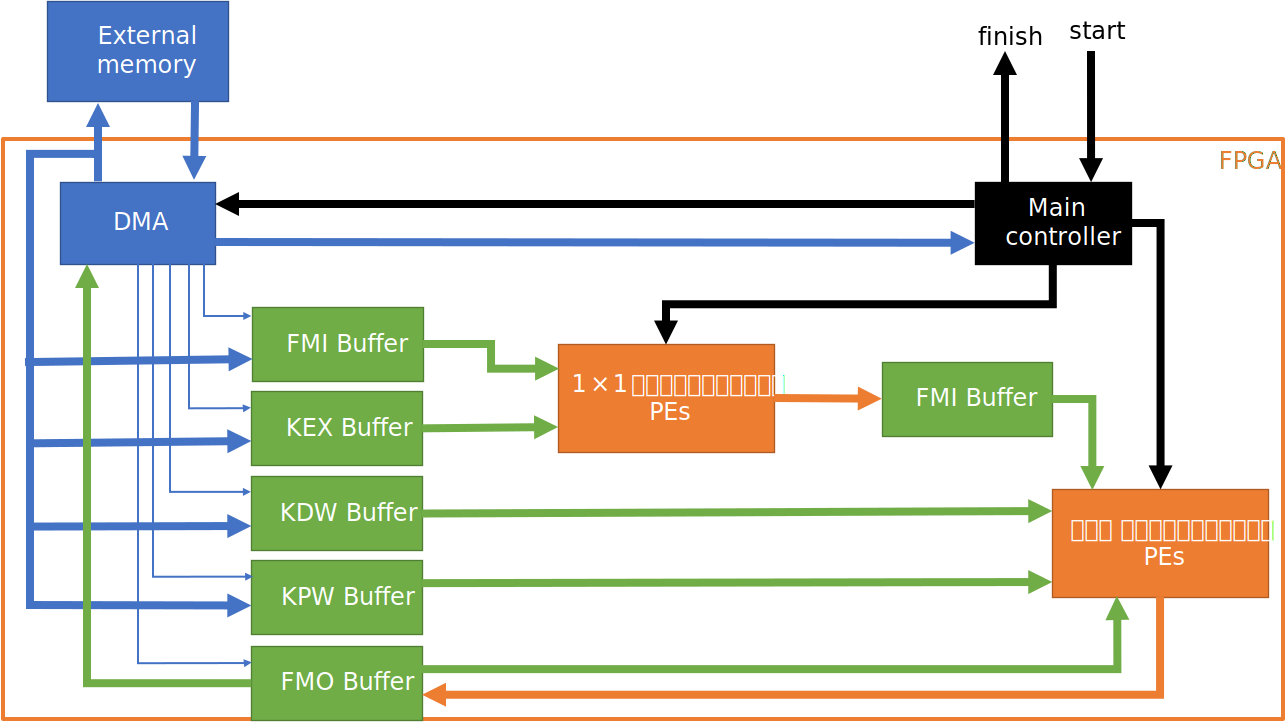
\includegraphics[width=\textwidth]{overal_archi.pdf}
    \caption{Overal architecture of the accelerator}
    \label{fig:overal_archi}
\end{figure}
%
An illustration of the overal architecture is illustrated in Figure \ref{fig:overal_archi}.
%
\subsection{Main controller}
